\chapter{Mathematics of TDA}\label{mathematicstda}

In this appendix, we include mathematical definitions, theorems, and examples from lecture notes taken at the Australian Mathematical Sciences Institute Summer School at Monash University in January 2026. Dr Daniele Celoria and Dr Agnese Barbensi from the University of Queensland lectured on ‘Computational and Combinatorial Algebraic Topology,’ which introduced the mathematical theory underpinning TDA.

\section{Simplicial Complexes}

\begin{definition}\label{simplicialcomplex}
    Let $n\in \mathbb{N}$. Define $[n] = \{0,1,\dots, n-1\}$. A \textit{simplicial complex} $X$ on $[n]$ is $X \subseteq \mathcal{P}([n])$ such that if $\sigma \in X$ and $\tau \leq \sigma$ then $\tau \in X$.
\end{definition}

\begin{definition}\label{dimsimplex}
     The \textit{dimension} of an $n-$simplex is $n$:
\[
\dim \Delta^n = n.
\]
The dimension of a simplicial complex is the dimension of the greatest $n-$simplex it contains.
\[
\dim X = \max \{n \mid \Delta^n \subseteq  X\}.
\]
\end{definition}

\begin{definition}\label{eulerch}
The \textit{Euler characteristic} is a function  from the set of simplicial complexes to the integers $\chi: S_{\text{spcx}}\rightarrow \mathbb{Z}$ given by:
\[
\chi(X) = \sum_{i\geq 0}(-1)^i \ |X_i|
\]
where $|X_i|$ is the number of simplices of dimension $n$ in $X$. Moreover, the Euler characteristic is a specialisation of the \textit{Poincare polynomial} $P: S_{\text{spcx}}\rightarrow \mathbb{Z}[t]$ at $t = -1$:
\[
P(t) = \sum_{i\geq 0}|X_i| t^i.
\]
For example, consider the $3-$simplex $\Delta^3$:
\[
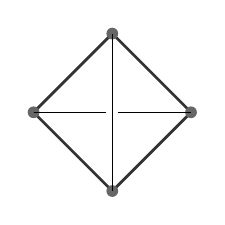
\begin{tikzpicture}[scale = 0.5, every node/.style={circle, fill=black!60, inner sep=1.5pt},
    vertex label/.style={font=\small\itshape, above right, fill = none},
    edge/.style={line width=1pt, black!80},
    face/.style={fill=gray!30, draw=none}
  ]

  % Coordinates
  \coordinate (x1) at (0,2);
  \coordinate (x2) at (2,0);
  \coordinate (x3) at (-2,0);
  \coordinate (x4) at (0,-2);
  
  % Edges
  \draw[edge] (x1) -- (x3) -- (x4) -- (x2) -- cycle;

  % Vertices
  \foreach \i in {1,2,3,4}
    \node (x\i) at (x\i) {};

  \draw (0,-2) -- (0,2);
  \draw (-2,0) -- (-0.15,0);
  \draw (0.15,0) -- (2,0);

\end{tikzpicture}
\]
It has one 3-dimensional simplex (the tetrahedron itself), four 2-dimensional simplices (the triangle faces), six 1-dimensional simplices (edges), and four 0-dimensional simplices (vertices). Therefore:
\[
\chi(\Delta^3) = 4 - 6 + 4 - 1 = 1.
\]
\end{definition}

\section{Chain Complexes and Homology}

\begin{definition}\label{chaincomplex}
    A \textit{chain complex} over $R$ (taken to be a ring with identity, usually $\mathbb{Z}, \mathbb{Q}, \mathbb{Z}/2\mathbb{Z}$) is a sequence of finitely generated $R-$modules $C_k, k\in \mathbb{Z}$ and morphisms $f_k: C_k \rightarrow C_{k-1}$ such that $f_k \circ f_{k+1} = 0$ for all $k$. 
\end{definition}

\begin{definition}\label{boundary}
    Given an oriented simplex $\Delta^n = [v_0, \dots, v_n]$, its \textit{algebraic boundary operator} is:
\[
\partial\Delta^n = \sum^n_{i=0} (-1)^i [v_0, \dots, \widehat{v}_i, \dots, v_n]
\]
where $\widehat{v}_i$ indicates that $v_i$ is removed, and the sum is treated as a purely formal sum.
\\\\
For example,
\[
\partial (\overset{v_0}{\circ} - \overset{v_1}{\circ}) = [v_0] - [v_1]
\]
and
\[
\partial
\bigg(\vcenter{\hbox{
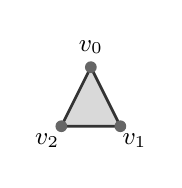
\begin{tikzpicture}[scale = 0.25, every node/.style={circle, fill=black!60, inner sep=1.5pt},
    vertex label/.style={font=\small\itshape, above right, fill = none},
    edge/.style={line width=1pt, black!80},
    face/.style={fill=gray!30, draw=none}
  ]

  % Coordinates
  \coordinate (x0) at (0,0);
  \coordinate (x1) at (1.5,3);
  \coordinate (x2) at (3,0);

  % Shaded triangle face
  \begin{scope}
    \path[face] (x0) -- (x1) -- (x2) -- cycle;
  \end{scope}
  
  % Edges
  \draw[edge] (x0) -- (x1) -- (x2) -- cycle;

  % Vertices
  \foreach \i in {0,1,2}
    \node (x\i) at (x\i) {};

  % Labels
  \node[vertex label, below left] at (x0) {$v_2$};
  \node[vertex label, above] at (x1) {$v_0$};
  \node[vertex label, below right] at (x2) {$v_1$};

\end{tikzpicture}
}}\bigg) = (\overset{v_1}{\circ} - \overset{v_2}{\circ}) + (\overset{v_0}{\circ} - \overset{v_1}{\circ}) - (\overset{v_2}{\circ} - \overset{v_0}{\circ}).
\]
\end{definition}

\begin{definition}\label{exactseq}
     If we have a sequence
\[
\dots \rightarrow C_{k+1} \overset{f_{k+1}}{\rightarrow} C_k \overset{f_k}{\rightarrow}C_{k-1} \dots
\]
we say it is exact in $k$ if 
\[
\ker f_k = \text{im}f_{k+1}
\]
which implies that $f_k \circ f_{k+1} = 0$.
\end{definition}

\begin{definition}\label{homgroup}
    Let $(C,f)$ be a chain complex. The \textit{homology group} of $(C,f)$ is the failure of exactness:
\[
H_k(C,f) = \frac{\ker f_k}{\text{im} f_{k+1}}.
\]
Remark: $(C,f)$ exact in $k$ implies that $H_k(C,f) = 0$. Moreover, one commonly regards $\ker f_k = Z_k$ as cycles and $\text{im} f_{k+1} = B_k$ as boundaries.
\end{definition}

\begin{definition}\label{chaingroup}
    If $X$ is a simplicial complex then 
\[
C_k(X) = \left\{\sum_i a_i \sigma_i \mid a_i \in \mathbb{Z}, \dim \sigma_i = K  \right\}
\]
is the \textit{simplicial chain group}, also known as the free group generated (over $\mathbb{Z}$) by the $K-$simplices. Moreover, 
\[
C(X) = \bigoplus_{k \in \mathbb{N}} C_k(X).
\]
\end{definition}

\begin{definition}\label{simhom}
     The \textit{simplicial homology} of $X$ is
\[
H(C(X), \partial) = H_* (X; \mathbb{Z}),
\]
where $*$ indicates that we may consider some $k$ or all of $k$. 
\end{definition}

\begin{example}\label{simhomexample}
    Consider the simplicial complex $\Delta^1$. Its chain complex is given by:
\[
\dots 0 \rightarrow C_1(X) \rightarrow C_0(X) \rightarrow 0 \dots
\]
Which equates to:
\[
\dots 0 \rightarrow \mathbb{Z}\langle[v_0,v_1]\rangle \overset{\partial_1}{\rightarrow} \mathbb{Z}\langle[v_0],[v_1]\rangle \rightarrow 0 \dots
\]
Now, we can compute $\partial_1: \mathbb{Z} \rightarrow \mathbb{Z}^2$ explicitly by
\[
\partial_1 = \begin{pmatrix}
    -1 \\ 1
\end{pmatrix}.
\]
The kernel of $\partial_1$ is given by $\ker \partial_1 = 0$, so $H_1(\Delta^1; \mathbb{Z})=0$. Moreover, the image of $\partial_1$ is given by $\text{im}(\partial_1) = - a[v_0]+a[v_1], a \in \mathbb{Z}$ so $\ker \partial_0 = \mathbb{Z}^2$. Thus, $H_0(\Delta^1; \mathbb{Z}) = \mathbb{Z}^2/\text{im}\partial_1 \cong \mathbb{Z}\langle[v_0]\rangle \cong \mathbb{Z}\langle[v_1]\rangle$. All in all,
\[
H_*(\Delta^1, \mathbb{Z}) = 
\begin{cases}
    \mathbb{Z} & * = 0 \\
    0 & \text{otherwise}
\end{cases}.
\]
\end{example}



\section{Persistent Homology}



\begin{definition}\label{filtration}
    Let $(C, \partial)$ be a chain complex. A \textit{filtration} on $C$ is:
\[
\varnothing = F_0C \subseteq F_1C \subseteq \dots \subseteq F_mC = C
\]
such that $\partial(F_kC) \subseteq F_k C$, meaning that each $F_kC$ is a subchain complex. If $X$ is a simplicial complex then $F_k X$ is the \textit{$k$-skeleton of $X$}.
\end{definition}

\begin{definition}\label{vrcomplex}
    Let $(M,d)$ be a finite metric space. Then, the \textit{Vietoris-Rips complex} $\text{VR}_\epsilon(M)$ has vertices given by the set $\{X_0,X_1,\dots,X_k\}\subset M$ and $k$-simplices are included if and only if $d(X_i,X_j)\leq \epsilon$ for all pairs.
\end{definition}

\begin{definition}\label{vrfiltration}
    The Vietoris–Rips filtration is the nested family of simplicial complexes:
\[
\{\text{VR}_\epsilon(M)\}_{\epsilon \geq 0},
\]
\end{definition}

\begin{definition}\label{persistencemodule}
    An $\mathbb{N}$-indexed \textit{persistence module} over a field $\mathbb{F}$ is a sequence $(V, a)$ of $\mathbb{F}$-vector spaces with linear maps between them:
\[
V_0 \overset{a_0}{\longrightarrow} V_1 \overset{a_1}{\longrightarrow}V_2 \overset{a_2}{\longrightarrow} V_3 \overset{a_3}{\longrightarrow}\dots
\]
We say that a persistence module is of finite type if $\dim V_i < \infty$ and $a_i$ is an isomorphism for large enough $i$. 
\end{definition}

\begin{definition}\label{persistencegroup}
    For $i,j \in \mathbb{N}, j \geq i $ the $i,j$ persistent homology group of the persistent module $(V,a)$ is the subspace of $V_j$ given by:
\[
\text{PH}_{ij}(V,a) = \text{im}(a_{ij}) \subset V_j,
\]
where $a_{ij}$ is shorthand for the composition $a_{j-1} \circ a_{j-2} \circ \dots \circ a_j : V_i \rightarrow V_j$.
\end{definition}

\begin{definition}\label{terminology}
    Several pieces of terminology are also commonplace:
\begin{itemize}
    \item A cycle $v \in V_i$ is \textit{born at filtration index i} if $v \notin \text{im}(a_{i-1})$,
    \item A cycle $v \in V_i$ is said to \textit{die at filtration index $j\geq i$} if $j$ is the smallest index such that $a_{ij}(v)=0$,
    \item If $a_{ij}(v)=0$ never occurs then the \textit{death time} of $v$ is $+\infty$,
    \item The \textit{persistence} of $v$ is $j-i$.
\end{itemize}
\end{definition}

\begin{definition}\label{intervalmod}
    For all $0\leq i \leq j \leq \infty$, $i\neq \infty$, the $\mathbb{N}$-indexed persistence module $(I^{i,j}, c^{i,j})$ given by:
\begin{align*}
    I^{i,j}_p &= 
    \begin{cases}
        \mathbb{F} & i \leq p \leq j \\
        0 & \text{otherwise} 
    \end{cases} \\
    c^{i,j}_p &= 
    \begin{cases}
        \text{id}_\mathbb{F} & i \leq p \leq j \\
        0 & \text{otherwise}
    \end{cases}
\end{align*}
is called an interval module.
\end{definition}


\begin{theorem}\label{structuretheorem}
    For any finite type $\mathbb{N}$-indexed persistence module $(V, a)$ over $\mathbb{F}$, there exists a set of integer pairs $0 \leq i \leq j \leq \infty$ (with $i\neq \infty$) such that there is a unique (up to isomorphism of persistence modules) direct sum decomposition:
\[
(V, a) \cong \bigoplus_{[i,j]}(I^{i,j}, c^{i,j}).
\]
\end{theorem}
\begin{proof}
See \cite[Theorem 6.9]{nanda_cat_notes}.   
\end{proof}

\begin{definition}\label{barcode}
The collection of intervals $[i,j]$ (with multiplicity) generated by the Structure Theorem is the \textit{barcode} of $(V, a)$.    
\end{definition}

\begin{definition}\label{epsinterleaving}
    For $\epsilon \geq 0$, an $\epsilon$-interleaving between $(V,a)$ and $(W,b)$ consists of two families of functions:
\begin{align*}
    &\{\phi_t: V_t \rightarrow W_{t+\epsilon} \mid t\geq 0\} \\
    &\{\psi_t: W_t \rightarrow V_{t+\epsilon} \mid t\geq 0\}
\end{align*}
with two requirements:
\begin{enumerate}
    \item The parallelogram law:
    \begin{enumerate}
        \item For all $s\leq t$, $\phi_t \circ a_{s\leq t} = b_{s+\epsilon \leq t + \epsilon} \circ \phi_s$.
        \item For all $s\leq t$, $\psi_t \circ b_{s\leq t} = a_{s+\epsilon \leq t+\epsilon}\circ \psi_s$.
    \end{enumerate}
    \item The triangle law:
    \begin{enumerate}
        \item For all $t$, $\psi_{t+\epsilon} \circ \phi_t = a_{t\leq t+ 2\epsilon}$.
        \item For all $t$, $\phi_{t+\epsilon} \circ \psi_t = b_{t\leq t+2\epsilon}$.
    \end{enumerate}
\end{enumerate}
\end{definition}

\begin{definition}\label{interleavingdist}
    The \textit{interleaving distance} $d((V,a), (W, b))$ is defined as the $\inf_\epsilon$ such that there exists an $\epsilon$-interleaving between $V$ and $W$.
\end{definition}

\begin{definition}\label{epsilonmatching}
     For $\epsilon \geq 0$ and $\epsilon$-matching between multisets $B,B'$ of intervals is $\rho: B_0 \rightarrow B^{'}_0$ a bijection with $B_0 \subset B$ and $B^{'}_0 \subset B'$ such that:
\begin{itemize}
    \item Every $[s,t]$ in $(B\setminus B_0) \cup (B'\setminus B^{'}_0)$ has length $t-s\leq 2\epsilon$.
    \item If $\rho[s,t]=[s',t']$ then $|s-s'|\leq \epsilon$ and $|t-t'| \leq \epsilon$.
\end{itemize}
\end{definition}

\begin{definition}\label{bottleneckdist}
    The bottleneck distance $d_B(B,B')$ is the infimum over all $\epsilon \geq 0$ such that there exists an $\epsilon$-matching between $B$ and $B'$.
\end{definition}

\begin{definition}\label{wassersteindist}
    Let $D, D'$ be persistence diagrams. Define the Wasserstein distance:
\[
d_{WP}(D,D') = \min_{m\in M(D,D')}\left(\sum_{(a,b)\in M}||a-b||^p_p + \sum||s-\text{Proj}(s)||^p_p  \right)^{1/p}.
\]
\end{definition}
